% Compile with LuaLaTeX:
%   lualatex -interaction=nonstopmode EXP_AUGUST_CLOSED_LOOP_FLOWCHART.tex
% The page is exactly 16:9. All module and node positions are explicit.
\documentclass[10pt]{article}
\usepackage[paperwidth=16in,paperheight=9in,margin=0in]{geometry}
\usepackage{fontspec}
\usepackage{tikz}
\usetikzlibrary{arrows.meta,backgrounds,calc,fit,positioning,shapes.geometric}
\pagestyle{empty}
\setmainfont{Arial}
\hyphenpenalty=10000
\exhyphenpenalty=10000

\definecolor{ink}{HTML}{172033}
\definecolor{muted}{HTML}{516070}
\definecolor{bluefill}{HTML}{EAF3FF}
\definecolor{bluestroke}{HTML}{2F6FB3}
\definecolor{greenfill}{HTML}{EAF8F0}
\definecolor{greenstroke}{HTML}{2E7D5B}
\definecolor{amberfill}{HTML}{FFF5DC}
\definecolor{amberstroke}{HTML}{A66B10}
\definecolor{orangefill}{HTML}{FFF0E6}
\definecolor{orangestroke}{HTML}{B85C2E}
\definecolor{purplefill}{HTML}{F2ECFF}
\definecolor{purplestroke}{HTML}{6842A8}
\definecolor{redfill}{HTML}{FDECEC}
\definecolor{redstroke}{HTML}{A34848}

% Boxes explain responsibilities; edge symbols carry the data semantics.
\newcommand{\tasktwo}[2]{{\fontsize{12}{13.8}\selectfont
    \textbullet\ #1\\\textbullet\ #2}}
\newcommand{\tasktwoleft}[2]{{\fontsize{12}{13.8}\selectfont
    \parbox{1.82in}{\raggedright
    \textbullet\ #1\\\textbullet\ #2}}}
\newcommand{\taskfour}[4]{{\fontsize{12}{13.8}\selectfont
    \textbullet\ #1\\\textbullet\ #2\\
    \textbullet\ #3\\\textbullet\ #4}}
\newcommand{\taskfourleft}[4]{{\fontsize{12}{13.8}\selectfont
    \parbox{1.72in}{\raggedright
    \textbullet\ #1\\\textbullet\ #2\\
    \textbullet\ #3\\\textbullet\ #4}}}
\newcommand{\taskkey}[3]{{\fontsize{12}{13.8}\selectfont
    \textbullet\ #1\\\textbullet\ #2\\
    \textcolor{orangestroke}{\bfseries KEY: #3}}}
\newcommand{\taskkeyleft}[3]{{\fontsize{12}{13.8}\selectfont
    \parbox{1.82in}{\raggedright
    \textbullet\ #1\\\textbullet\ #2\\
    \textcolor{orangestroke}{\bfseries KEY: #3}}}}
\newcommand{\taskkeywide}[3]{{\fontsize{12}{13.8}\selectfont
    \parbox{2.16in}{\raggedright
    \textbullet\ #1\\\textbullet\ #2\\
    \textcolor{orangestroke}{\bfseries KEY: #3}}}}
\newcommand{\nodeinfo}[1]{{\fontsize{12}{13.8}\selectfont #1}}

\begin{document}
\begin{tikzpicture}[
    remember picture,
    overlay,
    shift={(current page.south west)},
    x=1in,
    y=1in,
    every node/.style={font=\fontsize{12}{14}\selectfont,text=ink,align=center},
    box/.style={
        draw,
        rounded corners=5pt,
        line width=1.15pt,
        minimum height=1.04in,
        text width=2.02in,
        inner xsep=6pt,
        inner ysep=7pt,
        fill=white
    },
    source/.style={box,fill=bluefill,draw=bluestroke},
    observe/.style={box,fill=greenfill,draw=greenstroke},
    hypothesis/.style={box,fill=amberfill,draw=amberstroke},
    reasoning/.style={box,fill=orangefill,draw=orangestroke,text width=2.28in},
    frozen/.style={box,fill=purplefill,draw=purplestroke},
    evaluation/.style={box,fill=redfill,draw=redstroke},
    decision/.style={
        diamond,
        aspect=2.0,
        draw=amberstroke,
        fill=amberfill,
        line width=1.15pt,
        inner xsep=3pt,
        inner ysep=2pt,
        text width=1.44in,
        font=\fontsize{10.5}{12}\selectfont
    },
    flow/.style={-{Latex[length=3.2mm,width=2.0mm]},line width=1.35pt,draw=ink,rounded corners=7pt},
    feedback/.style={-{Latex[length=3.5mm,width=2.2mm]},line width=2.0pt,draw=amberstroke,rounded corners=9pt},
    readonly/.style={-{Latex[length=3.2mm,width=2.0mm]},line width=1.25pt,draw=redstroke,densely dashed,rounded corners=7pt},
    flowlabel/.style={
        fill=none,
        inner sep=0pt,
        font=\fontsize{14}{15}\selectfont
    },
    smalllabel/.style={flowlabel,font=\fontsize{11.5}{13}\selectfont},
    moduletitle/.style={font=\bfseries\fontsize{13.5}{15}\selectfont,anchor=west,text=ink},
    subtitle/.style={font=\fontsize{8.5}{10}\selectfont,text=muted}
]

% ---------------------------------------------------------------------------
% Fixed 16:9 frame and four fixed module quadrants.
% ---------------------------------------------------------------------------
\path[use as bounding box] (0,0) rectangle (16,9);
\node[font=\bfseries\fontsize{19}{22}\selectfont,anchor=north west]
    at (0.34,8.83) {Video-only Knowledge-constrained Closed-loop Inference};
\node[subtitle,anchor=north east]
    at (15.66,8.80) {No human segmentation is accessible before predictions are frozen};

\begin{scope}[on background layer]
    \filldraw[fill=bluefill!25,draw=bluestroke!60,line width=1.2pt,rounded corners=10pt]
        (0.30,4.70) rectangle (7.82,8.38);
    \filldraw[fill=amberfill!35,draw=amberstroke!65,line width=1.2pt,rounded corners=10pt]
        (8.18,4.70) rectangle (15.70,8.38);
    \filldraw[fill=purplefill!32,draw=purplestroke!65,line width=1.2pt,rounded corners=10pt]
        (0.30,0.78) rectangle (7.82,4.40);
    \filldraw[fill=amberfill!22,draw=amberstroke!65,line width=1.2pt,rounded corners=10pt]
        (8.18,0.78) rectangle (15.70,4.40);
\end{scope}

\node[moduletitle] at (0.52,8.19) {I · VIDEO $\rightarrow$ OBSERVATIONS};
\node[moduletitle] at (8.40,8.19) {II · INITIAL STATE $\rightarrow$ CONSTRAINTS};
\node[moduletitle] at (0.52,4.21) {IV · FREEZE $\rightarrow$ BLIND EVALUATION};
\node[moduletitle] at (8.40,4.21) {III · RE-ESTIMATE $\rightarrow$ SELECT};

% ---------------------------------------------------------------------------
% Module I — upper left. Explicit serpentine path prevents central overlaps.
% ---------------------------------------------------------------------------
\node[source,text width=1.72in] (video) at (1.35,7.43)
    {\textbf{Raw Video}\\[4pt]\tasktwo{decode RGB frames}{preserve timing}};
\node[source,text width=1.72in] (knowledge) at (1.35,6.28)
    {\textbf{Frozen Knowledge}\\[4pt]\tasktwo{encode physics priors}{freeze rule set}};
\node[observe] (s1) at (4.15,7.43)
    {\textbf{Step 1 · Init}\\[4pt]
     \tasktwoleft{Video Validation}{Timeline Normalization}};
\node[observe] (s2) at (6.63,7.27)
    {\textbf{Step 2 · Neural Perception}\\[4pt]
     \taskfourleft{Objects (YOLO)}{Masks (SAM 2)}{Optical Flow (RAFT)}{Depth (DA3)}};
\node[observe,text width=2.36in] (s3) at (3.95,5.54)
    {\textbf{Step 3 · Object Tracking}\\[4pt]
     \nodeinfo{\parbox{2.16in}{\raggedright\textbullet\ Build ID consistent mask tracks}}};
\node[observe] (s4) at (6.63,5.54)
    {\textbf{Step 4 · Geometry/Scale}\\[4pt]
     \taskkeyleft{recover camera pose}{resolve metric scale}{multi-cue geometry}};

\draw[flow] (video.east) .. controls +(0.65,0.08) and +(-0.58,0.26) ..
    node[flowlabel,pos=0.47,yshift=10pt] {$\mathcal{X}$} (s1.north west);
\draw[flow] (knowledge.east) .. controls +(0.68,0.00) and +(-0.62,-0.26) ..
    node[flowlabel,pos=0.48,yshift=-12pt] {$\mathcal{K}$} (s1.south west);
\draw[flow] (s1.east) -- node[flowlabel,above=8pt] {$\mathcal{M}$} (s2.west);
\draw[flow] (s2.south) .. controls +(-0.58,-0.33) and +(0.72,0.30) ..
    node[flowlabel,pos=0.48,yshift=12pt] {$\mathcal{O}_t$} (s3.north);
\draw[flow] (s3.east) -- node[flowlabel,above=8pt] {$\mathcal{T}$} (s4.west);

% ---------------------------------------------------------------------------
% Module II — upper right.
% ---------------------------------------------------------------------------
\node[hypothesis] (s5) at (9.48,7.19)
    {\textbf{Step 5 · Joint State}\\[4pt]
     \tasktwoleft{fuse ego + object states}{initialize world models}};
\node[hypothesis] (beam) at (11.94,7.19)
    {\textbf{Top-K Hypotheses}\\[4pt]
     \tasktwo{preserve alternatives}{retain uncertainty}};
\node[hypothesis] (s6) at (14.40,7.19)
    {\textbf{Step 6 · Consistency}\\[4pt]
     \taskkeyleft{compute residuals}{test temporal coherence}{physical plausibility}};
\node[hypothesis] (s7) at (9.55,5.55)
    {\textbf{Step 7 · Evidence Check}\\[4pt]
     \taskkeyleft{sample keyframes}{localize conflicts}{logic checks}};
\node[reasoning] (repair) at (12.48,5.55)
    {\textbf{Knowledge + Numerical Repair}\\[4pt]
     \taskkey{propose bounded repairs}{solve parameters}{LLM + numeric solver}};

\draw[flow] (s5.east) -- node[flowlabel,above=8pt] {$\mathcal{H}_0$} (beam.west);
\draw[flow] (beam.east) -- node[flowlabel,above=8pt] {$\mathcal{B}_i$} (s6.west);
\draw[flow] (s6.south) -- ++(0,-0.34) -| node[flowlabel,pos=0.56,above=11pt] {$\mathcal{R}_i$} (s7.north);
\draw[flow] (s7.east) -- node[flowlabel,above=8pt] {$\mathcal{E}_i$} (repair.west);

% Module I -> II. The label is shifted above the inter-module bridge.
\draw[flow] (s4.east) -- ++(0.30,0) |- node[smalllabel,pos=0.42,yshift=11pt]
    {$\bigl(\mathcal{G},\mathcal{O}_t,\mathcal{K}\bigr)$} (s5.west);

% ---------------------------------------------------------------------------
% Module III — lower right.
% ---------------------------------------------------------------------------
\node[hypothesis] (s8) at (9.48,3.28)
    {\textbf{Step 8 · Local Re-estimation}\\[4pt]
     \tasktwoleft{re-estimate local windows}{generate variants}};
\node[hypothesis] (s9) at (11.94,3.28)
    {\textbf{Step 9 · Unified Score}\\[4pt]
     \tasktwoleft{enforce hard constraints}{rank soft residuals}};
\node[hypothesis] (best) at (14.40,3.28)
    {\textbf{Best-ever Register}\\[4pt]
     \tasktwo{retain the Top-K beam}{track best-ever score}};
\node[decision] (stop) at (9.48,1.62)
    {\textbf{Stop?}\\[4pt]\tasktwo{constraints pass}{$\Delta J_i\leq\varepsilon$ or budget}};
\node[hypothesis,text width=2.10in] (loopback) at (12.48,1.62)
    {\textbf{Feedback Return}\\[4pt]
     \tasktwo{form the next beam}{preserve provenance}};

\draw[flow] (s8.east) -- node[smalllabel,above=9pt] {$\mathcal{H}_{i+1}^{1:n}$} (s9.west);
\draw[flow] (s9.east) -- node[flowlabel,above=8pt] {$\mathcal{Q}_i$} (best.west);
\draw[flow] (best.south) -- ++(0,-0.31) -| node[smalllabel,pos=0.32,right=8pt]
    {$\mathcal{H}^{*},\Delta J_i$} (stop.east);
\draw[feedback] (stop.east) -- node[smalllabel,above=9pt] {$C_i=0$} (loopback.west);
\draw[feedback]
    (loopback.east) -- (15.57,1.62) -- (15.57,7.86)
    -- (11.94,7.86)
    -- (beam.north);
\node[smalllabel] at (13.75,8.01) {$\mathcal{B}_{i+1}$};

% Module II -> III.
\draw[flow] (repair.south) -- ++(0,-0.34) -| node[flowlabel,pos=0.46,above=11pt]
    {$\Delta_i$} (s8.north);

% ---------------------------------------------------------------------------
% Module IV — lower left. Flow proceeds right-to-left, matching the 2x2 cycle.
% ---------------------------------------------------------------------------
\node[frozen] (freeze) at (6.62,3.20)
    {\textbf{Freeze Best Explanation}\\[4pt]
     \taskkey{lock the best hypothesis}{seal inference artifacts}{leakage-free freeze}};
\node[frozen] (s10) at (4.15,3.20)
    {\textbf{Step 10 · Segmentation}\\[4pt]
     \tasktwoleft{locate change points}{assign segment labels}};
\node[frozen] (s11) at (1.66,3.20)
    {\textbf{Step 11 · Symbolic Scene}\\[4pt]
     \tasktwoleft{build scene atoms}{attach provenance}};
\node[frozen] (pred) at (1.66,1.55)
    {\textbf{Frozen Predictions}\\[4pt]
     \tasktwo{export JSON + CSV}{render video + manifest}};
\node[evaluation] (eval) at (4.15,1.55)
    {\textbf{Independent Evaluator}\\[4pt]
     \tasktwo{measure F1 + tIoU}{analyze confusion}};
\node[evaluation] (ann) at (6.62,1.55)
    {\textbf{Human Segmentation}\\[4pt]
     \taskkey{provide reference labels}{support blind evaluation}{held-out labels}};

\draw[flow] (freeze.west) -- node[flowlabel,above=8pt] {$\mathcal{W}^{*}$} (s10.east);
\draw[flow] (s10.west) -- node[flowlabel,above=8pt] {$\mathcal{Z}^{*}$} (s11.east);
\draw[flow] (s11.south) -- node[flowlabel,right=8pt] {$\mathcal{A}^{*}$} (pred.north);
\draw[readonly] (pred.east) -- node[flowlabel,above=8pt] {$\mathcal{P}^{*}$} (eval.west);
\draw[readonly] (ann.west) -- node[flowlabel,above=8pt] {$\mathcal{Y}$} (eval.east);

% Module III -> IV. Short bridge across the central gutter.
\draw[flow] (stop.west) -- ++(-0.30,0) |- (freeze.east);
\node[smalllabel] at (8.02,3.39) {$C_i=1:\ \mathcal{H}^{*}$};

% ---------------------------------------------------------------------------
% Compact notation strip. Full definitions remain in the companion Markdown.
% ---------------------------------------------------------------------------
\node[anchor=south west,font=\fontsize{12}{13.8}\selectfont,text=muted,align=left]
at (0.38,0.38) {%
$\mathcal{X}$ video · $\mathcal{K}$ knowledge · $\mathcal{O}_t$ neural evidence ·
$\mathcal{T}$ ID-aligned masklets · $\mathcal{G}$ geometry · $\mathcal{B}_i$ beam ·
$\mathcal{R}_i$ residuals · $\mathcal{E}_i$ evidence};
\node[anchor=south west,font=\fontsize{12}{13.8}\selectfont,text=muted,align=left]
at (0.38,0.11) {%
$\Delta_i$ repairs · $\mathcal{H}^{*}$ best explanation · $\mathcal{W}^{*}$ frozen world ·
$\mathcal{Z}^{*}$ segments · $\mathcal{A}^{*}$ symbolic scene ·
$\mathcal{P}^{*}$ predictions · $\mathcal{Y}$ human labels};

\end{tikzpicture}
\end{document}
